%%%%%%%%%%%%%%%%%%%%%%%%%%%%%%%%%%%%%%%%%%%%%%%%%%%%%%%%%%%%%%%%%%%%%%%%%%%%%%%%%%%%%%%%%%%%%%%%%%%
%%%%%%%%%%%%%%%%%%%%%%%%%%%%%%%%%%%%%%%%%%%%%%%%%%%%%%%%%%%%%%%%%%%%%%%%%%%%%%%%%%%%%%%%%%%%%%%%%%%
\chapter{Tablas y gr\'aficos}

En este ap\'endice se incluyen las gr\'aficas y tablas obtenidas durante el trabajo; en las 
diferentes secciones del texto 
puede hallarse una descripci\'on m\'as extensa de las tablas,
% a aocontinucai\'on, 
c\'omo se
calcularon y que significan, as\'i algunas posibles interpretaciones.

A modo de resumen, las tablas tienen la informaci\'on citada en la seccci\'on de resultados sobre
la cantidad de \'epocas\footnote{Una \'epoca contempla 30 segundos de registro, siguiendo las
recomendaciones de la AASM\cite{AASM07}} para las cuales el test PSR no-puede rechazar la
hip\'otesis de que son estacionarias ($\alpha < 0.05$) por lo que son referidas como
\textit{Posiblemente Estacionarias} (PE); 
se consideran por separado el total de \'epocas, las \'epocas clasificadas dentro del sue\~no MOR,
y sue\~no que no fue clasificado como MOR --para tener una muestra del sue\~no exluyente con 
respecto a las \'epocas MOR.
Como normalizaci\'on, tambi\'en se usa la proporci\'on de \'epocas PE en cada grupo.

Por otro lado, los gr\'aficos siguientes son aquellos citados en la secci\'on de discusi\'on,
y representan la distribuci\'on temporal y pseudo-espacial de las \'epocas PE dentro del PSG.


%%%%%%%%%%%%%%%%%%%%%%%%%%%%%%%%%%%%%%%%%%%%%%%%%

\begin{SidewaysFigure}
\centering
\begin{tabular}{c|ccccc|cccc|ccc}
& VCR & MJH & JAE & GHA & MFGR
& CLO & RLO & RRU & JGZ
& FGH & MGG & EMT \\
\hline
C3&6&18&10&1&12&6&35&16&1&2&28&22 \\
C4&7&16&4&2&10&4&40&5&0&1&23&26 \\
CZ&2&16&13&2&8&5&22&4&1&1&13&19 \\
F3&5&23&10&0&3&7&43&3&3&6&14&20 \\
F4&11&23&5&1&1&6&36&5&0&0&4&24 \\
F7&5&15&2&0&4&1&18&0&0&0&2&24 \\
F8&4&11&6&1&3&4&23&1&0&0&2&20 \\
FP1&2&7&1&0&1&0&0&1&0&22&0&22 \\
FP2&1&6&3&0&2&1&15&1&0&0&1&18 \\
FZ&11&18&19&0&6&7&38&2&2&0&20&23 \\
O1&10&20&5&3&23&2&25&9&2&5&18&19 \\
O2&13&23&3&3&21&3&34&9&1&1&12&16 \\
P3&6&17&2&2&26&5&33&8&0&1&24&17 \\
P4&4&19&4&5&18&4&27&5&1&4&15&21 \\
PZ&4&15&5&3&22&4&32&4&0&1&8&20 \\
T3&10&29&1&8&26&10&34&4&0&2&29&31 \\
T4&12&20&2&3&21&3&35&6&1&0&10&17 \\
T5&10&26&0&3&27&5&34&5&2&2&31&19 \\
T6&15&18&3&15&20&3&24&4&2&0&9&19 \\
LOG&6&20&8&0&9&5&11&2&0&1&8&30 \\
ROG&6&21&17&2&11&9&7&4&1&0&19&33 \\
EMG&14&11&0&0&17&14&16&4&0&0&3&7 \\
\hline
Total&73&127&171&55&95&132&99&38&33&22&166&47
\end{tabular}
\caption{Total de \'epocas PE clasificadas como sue\~no MOR 
(fase R) para cada
canal. %Se incluyen las medias y desviaciones est\'andar estimadas para los grupos 
%Control (izquierda) y PDC (centro).
}
\label{total_gpos_mor}
\end{SidewaysFigure}

\begin{SidewaysFigure}
\centering
\begin{tabular}{c|ccccc|cccc|ccc}
& VCR & MJH & JAE & GHA & MFGR
& CLO & RLO & RRU & JGZ
& FGH & MGG & EMT \\
\hline
C3&187&135&100&175&112&55&153&76&56&16&201&478 \\
C4&168&129&89&156&87&36&135&94&47&7&207&598 \\
CZ&167&131&88&107&77&54&145&69&62&8&180&518 \\
F3&168&134&83&150&73&57&175&79&68&107&143&331 \\
F4&180&132&55&146&24&41&135&80&49&0&137&549 \\
F7&158&137&77&213&87&45&112&68&58&0&152&262 \\
F8&157&123&30&168&36&41&96&86&48&0&128&574 \\
FP1&163&75&23&128&65&34&0&71&44&381&169&518 \\
FP2&156&82&44&116&21&33&99&26&44&0&146&449 \\
FZ&170&134&78&156&51&55&163&91&65&0&177&533 \\
O1&202&174&51&295&175&48&150&92&96&20&140&675 \\
O2&166&165&63&247&173&32&136&70&106&22&161&573 \\
P3&175&122&53&288&132&72&147&108&95&29&212&490 \\
P4&180&136&108&252&140&56&135&110&73&18&206&495 \\
PZ&156&131&90&216&112&57&167&112&59&15&177&497 \\
T3&181&140&52&230&171&81&112&80&102&27&115&603 \\
T4&181&121&35&182&128&26&110&112&87&10&122&531 \\
T5&218&146&16&265&199&78&137&104&61&19&208&621 \\
T6&218&148&49&194&181&38&118&98&84&18&209&558 \\
LOG&236&224&214&287&170&144&185&128&225&50&437&820 \\
ROG&236&205&212&334&159&126&179&110&225&67&455&873 \\
EMG&94&62&16&1&157&20&82&110&10&1&55&266 \\
\hline
Total&788&905&736&1038&727&812&747&376&1174&383&864&1376
\end{tabular}
\caption{Total  de \'epocas PE dentro del registro pero que no fueron clasificadas
como MOR (fases W y N) para cada
canal. %Se incluyen las medias y desviaciones est\'andar estimadas para los grupos 
%Control (izquierda) y PDC (centro).
}
\label{total_gpos_nmor}
\end{SidewaysFigure}

\begin{SidewaysFigure}
\centering
\begin{tabular}{c|ccccc|cccc|ccc}
& VCR & MJH & JAE & GHA & MFGR
& CLO & RLO & RRU & JGZ
& FGH & MGG & EMT \\
\hline
C3&193&153&110&176&124&61&188&92&57&18&229&500 \\
C4&175&145&93&158&97&40&175&99&47&8&230&624 \\
CZ&169&147&101&109&85&59&167&73&63&9&193&537 \\
F3&173&157&93&150&76&64&218&82&71&113&157&351 \\
F4&191&155&60&147&25&47&171&85&49&0&141&573 \\
F7&163&152&79&213&91&46&130&68&58&0&154&286 \\
F8&161&134&36&169&39&45&119&87&48&0&130&594 \\
FP1&165&82&24&128&66&34&0&72&44&403&169&540 \\
FP2&157&88&47&116&23&34&114&27&44&0&147&467 \\
FZ&181&152&97&156&57&62&201&93&67&0&197&556 \\
O1&212&194&56&298&198&50&175&101&98&25&158&694 \\
O2&179&188&66&250&194&35&170&79&107&23&173&589 \\
P3&181&139&55&290&158&77&180&116&95&30&236&507 \\
P4&184&155&112&257&158&60&162&115&74&22&221&516 \\
PZ&160&146&95&219&134&61&199&116&59&16&185&517 \\
T3&191&169&53&238&197&91&146&84&102&29&144&634 \\
T4&193&141&37&185&149&29&145&118&88&10&132&548 \\
T5&228&172&16&268&226&83&171&109&63&21&239&640 \\
T6&233&166&52&209&201&41&142&102&86&18&218&577 \\
LOG&242&244&222&287&179&149&196&130&225&51&445&850 \\
ROG&242&226&229&336&170&135&186&114&226&67&474&906 \\
EMG&108&73&16&1&174&34&98&114&10&1&58&273 \\
\hline
Total&861&1032&907&1093&822&944&846&414&1207&405&1030&1423
\end{tabular}
\caption{Total de \'epocas PE registradas
(todas las fases) para cada
canal. 
%Se incluyen las medias y desviaciones est\'andar estimadas para los grupos 
%Control (izquierda) y PDC (centro).
}
\label{total_gpos_total}
\end{SidewaysFigure}






%\begin{comment}
\begin{SidewaysFigure}
\centering
\begin{tabular}{c||ccccc|cc||cccc|cc||ccc}
& VCR & MJH & JAE & GHA & MFGR &$\widehat{\mu}$ & $\widehat{\sigma}$
& CLO & RLO & RRU & JGZ &$\widehat{\mu}$ & $\widehat{\sigma}$
& FGH & MGG & EMT \\
\hline
C3&0.082&0.142&0.058&0.018&0.126&0.085&0.050&0.045&0.354&0.421&0.030&0.213&0.204&0.091&0.169&0.468 \\
C4&0.096&0.126&0.023&0.036&0.105&0.077&0.045&0.030&0.404&0.132&0.000&0.141&0.184&0.045&0.139&0.553 \\
CZ&0.027&0.126&0.076&0.036&0.084&0.070&0.040&0.038&0.222&0.105&0.030&0.099&0.089&0.045&0.078&0.404 \\
F3&0.068&0.181&0.058&0.000&0.032&0.068&0.069&0.053&0.434&0.079&0.091&0.164&0.181&0.273&0.084&0.426 \\
F4&0.151&0.181&0.029&0.018&0.011&0.078&0.081&0.045&0.364&0.132&0.000&0.135&0.162&0.000&0.024&0.511 \\
F7&0.068&0.118&0.012&0.000&0.042&0.048&0.047&0.008&0.182&0.000&0.000&0.047&0.090&0.000&0.012&0.511 \\
F8&0.055&0.087&0.035&0.018&0.032&0.045&0.027&0.030&0.232&0.026&0.000&0.072&0.108&0.000&0.012&0.426 \\
FP1&0.027&0.055&0.006&0.000&0.011&0.020&0.022&0.000&0.000&0.026&0.000&0.007&0.013&1.000&0.000&0.468 \\
FP2&0.014&0.047&0.018&0.000&0.021&0.020&0.017&0.008&0.152&0.026&0.000&0.046&0.071&0.000&0.006&0.383 \\
FZ&0.151&0.142&0.111&0.000&0.063&0.093&0.062&0.053&0.384&0.053&0.061&0.138&0.164&0.000&0.120&0.489 \\
O1&0.137&0.157&0.029&0.055&0.242&0.124&0.085&0.015&0.253&0.237&0.061&0.141&0.121&0.227&0.108&0.404 \\
O2&0.178&0.181&0.018&0.055&0.221&0.130&0.089&0.023&0.343&0.237&0.030&0.158&0.158&0.045&0.072&0.340 \\
P3&0.082&0.134&0.012&0.036&0.274&0.108&0.104&0.038&0.333&0.211&0.000&0.145&0.155&0.045&0.145&0.362 \\
P4&0.055&0.150&0.023&0.091&0.189&0.102&0.068&0.030&0.273&0.132&0.030&0.116&0.115&0.182&0.090&0.447 \\
PZ&0.055&0.118&0.029&0.055&0.232&0.098&0.082&0.030&0.323&0.105&0.000&0.115&0.146&0.045&0.048&0.426 \\
T3&0.137&0.228&0.006&0.145&0.274&0.158&0.103&0.076&0.343&0.105&0.000&0.131&0.148&0.091&0.175&0.660 \\
T4&0.164&0.157&0.012&0.055&0.221&0.122&0.086&0.023&0.354&0.158&0.030&0.141&0.155&0.000&0.060&0.362 \\
T5&0.137&0.205&0.000&0.055&0.284&0.136&0.114&0.038&0.343&0.132&0.061&0.143&0.139&0.091&0.187&0.404 \\
T6&0.205&0.142&0.018&0.273&0.211&0.170&0.097&0.023&0.242&0.105&0.061&0.108&0.096&0.000&0.054&0.404 \\
LOG&0.082&0.157&0.047&0.000&0.095&0.076&0.058&0.038&0.111&0.053&0.000&0.050&0.046&0.045&0.048&0.638 \\
ROG&0.082&0.165&0.099&0.036&0.116&0.100&0.047&0.068&0.071&0.105&0.030&0.069&0.031&0.000&0.114&0.702 \\
EMG&0.192&0.087&0.000&0.000&0.179&0.091&0.093&0.106&0.162&0.105&0.000&0.093&0.068&0.000&0.018&0.149
\end{tabular}
\caption{Proporci\'on estimada de \'epocas PE respecto al total de \'epocas MOR 
(fase R) para cada
canal. Se incluyen las medias y desviaciones est\'andar estimadas para los grupos 
Control (izquierda) y PDC (centro).}
\label{gpos_mor}
\end{SidewaysFigure}

\begin{SidewaysFigure}
\centering
\begin{tabular}{c||ccccc|cc||cccc|cc||ccc}
& VCR & MJH & JAE & GHA & MFGR &$\widehat{\mu}$ & $\widehat{\sigma}$
& CLO & RLO & RRU & JGZ &$\widehat{\mu}$ & $\widehat{\sigma}$
& FGH & MGG & EMT \\
\hline
C3&0.237&0.149&0.136&0.169&0.154&0.169&0.040&0.068&0.205&0.202&0.048&0.131&0.085&0.042&0.233&0.347 \\
C4&0.213&0.143&0.121&0.150&0.120&0.149&0.038&0.044&0.181&0.250&0.040&0.129&0.104&0.018&0.240&0.435 \\
CZ&0.212&0.145&0.120&0.103&0.106&0.137&0.045&0.067&0.194&0.184&0.053&0.124&0.075&0.021&0.208&0.376 \\
F3&0.213&0.148&0.113&0.145&0.100&0.144&0.044&0.070&0.234&0.210&0.058&0.143&0.092&0.279&0.166&0.241 \\
F4&0.228&0.146&0.075&0.141&0.033&0.125&0.075&0.050&0.181&0.213&0.042&0.121&0.088&0.000&0.159&0.399 \\
F7&0.201&0.151&0.105&0.205&0.120&0.156&0.046&0.055&0.150&0.181&0.049&0.109&0.066&0.000&0.176&0.190 \\
F8&0.199&0.136&0.041&0.162&0.050&0.117&0.070&0.050&0.129&0.229&0.041&0.112&0.087&0.000&0.148&0.417 \\
FP1&0.207&0.083&0.031&0.123&0.089&0.107&0.065&0.042&0.000&0.189&0.037&0.067&0.083&0.995&0.196&0.376 \\
FP2&0.198&0.091&0.060&0.112&0.029&0.098&0.064&0.041&0.133&0.069&0.037&0.070&0.044&0.000&0.169&0.326 \\
FZ&0.216&0.148&0.106&0.150&0.070&0.138&0.055&0.068&0.218&0.242&0.055&0.146&0.098&0.000&0.205&0.387 \\
O1&0.256&0.192&0.069&0.284&0.241&0.209&0.085&0.059&0.201&0.245&0.082&0.147&0.090&0.052&0.162&0.491 \\
O2&0.211&0.182&0.086&0.238&0.238&0.191&0.063&0.039&0.182&0.186&0.090&0.124&0.072&0.057&0.186&0.416 \\
P3&0.222&0.135&0.072&0.277&0.182&0.178&0.079&0.089&0.197&0.287&0.081&0.163&0.098&0.076&0.245&0.356 \\
P4&0.228&0.150&0.147&0.243&0.193&0.192&0.044&0.069&0.181&0.293&0.062&0.151&0.109&0.047&0.238&0.360 \\
PZ&0.198&0.145&0.122&0.208&0.154&0.165&0.036&0.070&0.224&0.298&0.050&0.160&0.120&0.039&0.205&0.361 \\
T3&0.230&0.155&0.071&0.222&0.235&0.182&0.070&0.100&0.150&0.213&0.087&0.137&0.057&0.070&0.133&0.438 \\
T4&0.230&0.134&0.048&0.175&0.176&0.152&0.068&0.032&0.147&0.298&0.074&0.138&0.117&0.026&0.141&0.386 \\
T5&0.277&0.161&0.022&0.255&0.274&0.198&0.109&0.096&0.183&0.277&0.052&0.152&0.099&0.050&0.241&0.451 \\
T6&0.277&0.164&0.067&0.187&0.249&0.189&0.082&0.047&0.158&0.261&0.072&0.134&0.097&0.047&0.242&0.406 \\
LOG&0.299&0.248&0.291&0.276&0.234&0.270&0.028&0.177&0.248&0.340&0.192&0.239&0.074&0.131&0.506&0.596 \\
ROG&0.299&0.227&0.288&0.322&0.219&0.271&0.046&0.155&0.240&0.293&0.192&0.220&0.060&0.175&0.527&0.634 \\
EMG&0.119&0.069&0.022&0.001&0.216&0.085&0.086&0.025&0.110&0.293&0.009&0.109&0.130&0.003&0.064&0.193
\end{tabular}
\caption{Proporci\'on estimada de \'epocas PE respecto al total de \'epocas no-MOR 
(fases W y N) para cada
canal. Se incluyen las medias y desviaciones est\'andar estimadas para los grupos 
Control (izquierda) y PDC (centro).}
\label{gpos_nmor}
\end{SidewaysFigure}

\begin{SidewaysFigure}
\centering
\begin{tabular}{c||ccccc|cc||cccc|cc||ccc}
& VCR & MJH & JAE & GHA & MFGR &$\widehat{\mu}$ & $\widehat{\sigma}$
& CLO & RLO & RRU & JGZ &$\widehat{\mu}$ & $\widehat{\sigma}$
& FGH & MGG & EMT \\
\hline
C3&0.224&0.148&0.121&0.161&0.151&0.161&0.038&0.065&0.222&0.222&0.047&0.139&0.096&0.044&0.222&0.351 \\
C4&0.203&0.141&0.103&0.145&0.118&0.142&0.038&0.042&0.207&0.239&0.039&0.132&0.106&0.020&0.223&0.439 \\
CZ&0.196&0.142&0.111&0.100&0.103&0.131&0.040&0.063&0.197&0.176&0.052&0.122&0.075&0.022&0.187&0.377 \\
F3&0.201&0.152&0.103&0.137&0.092&0.137&0.043&0.068&0.258&0.198&0.059&0.146&0.098&0.279&0.152&0.247 \\
F4&0.222&0.150&0.066&0.134&0.030&0.121&0.075&0.050&0.202&0.205&0.041&0.124&0.092&0.000&0.137&0.403 \\
F7&0.189&0.147&0.087&0.195&0.111&0.146&0.047&0.049&0.154&0.164&0.048&0.104&0.064&0.000&0.150&0.201 \\
F8&0.187&0.130&0.040&0.155&0.047&0.112&0.065&0.048&0.141&0.210&0.040&0.110&0.081&0.000&0.126&0.417 \\
FP1&0.192&0.079&0.026&0.117&0.080&0.099&0.061&0.036&0.000&0.174&0.036&0.062&0.077&0.995&0.164&0.379 \\
FP2&0.182&0.085&0.052&0.106&0.028&0.091&0.059&0.036&0.135&0.065&0.036&0.068&0.046&0.000&0.143&0.328 \\
FZ&0.210&0.147&0.107&0.143&0.069&0.135&0.052&0.066&0.238&0.225&0.056&0.146&0.099&0.000&0.191&0.391 \\
O1&0.246&0.188&0.062&0.273&0.241&0.202&0.084&0.053&0.207&0.244&0.081&0.146&0.093&0.062&0.153&0.488 \\
O2&0.208&0.182&0.073&0.229&0.236&0.186&0.066&0.037&0.201&0.191&0.089&0.129&0.080&0.057&0.168&0.414 \\
P3&0.210&0.135&0.061&0.265&0.192&0.173&0.078&0.082&0.213&0.280&0.079&0.163&0.100&0.074&0.229&0.356 \\
P4&0.214&0.150&0.123&0.235&0.192&0.183&0.046&0.064&0.191&0.278&0.061&0.149&0.105&0.054&0.215&0.363 \\
PZ&0.186&0.141&0.105&0.200&0.163&0.159&0.038&0.065&0.235&0.280&0.049&0.157&0.118&0.040&0.180&0.363 \\
T3&0.222&0.164&0.058&0.218&0.240&0.180&0.074&0.096&0.173&0.203&0.085&0.139&0.058&0.072&0.140&0.446 \\
T4&0.224&0.137&0.041&0.169&0.181&0.150&0.069&0.031&0.171&0.285&0.073&0.140&0.113&0.025&0.128&0.385 \\
T5&0.265&0.167&0.018&0.245&0.275&0.194&0.107&0.088&0.202&0.263&0.052&0.151&0.098&0.052&0.232&0.450 \\
T6&0.271&0.161&0.057&0.191&0.245&0.185&0.083&0.043&0.168&0.246&0.071&0.132&0.093&0.044&0.212&0.405 \\
LOG&0.281&0.236&0.245&0.263&0.218&0.249&0.024&0.158&0.232&0.314&0.186&0.222&0.068&0.126&0.432&0.597 \\
ROG&0.281&0.219&0.252&0.307&0.207&0.253&0.042&0.143&0.220&0.275&0.187&0.206&0.056&0.165&0.460&0.637 \\
EMG&0.125&0.071&0.018&0.001&0.212&0.085&0.086&0.036&0.116&0.275&0.008&0.109&0.120&0.002&0.056&0.192
\end{tabular}
\caption{Proporci\'on estimada de \'epocas PE respecto al total de \'epocas registradas
(todas las fases) para cada
canal. Se incluyen las medias y desviaciones est\'andar estimadas para los grupos 
Control (izquierda) y PDC (centro).}
\label{gpos_total}
\end{SidewaysFigure}
%\end{comment}

%%%%%%%%%%%%%%%%%%%%%%%%%%%%%%%%%%%%%%%%%%%%%%%%%%%%%%%%%%%%%%%%%%%%%%%%%%%%%%%%%%%%%%%%%%%%%%%%%%%
%%%%%%%%%%%%%%%%%%%%%%%%%%%%%%%%%%%%%%%%%%%%%%%%%%%%%%%%%%%%%%%%%%%%%%%%%%%%%%%%%%%%%%%%%%%%%%%%%%%

\begin{figure}
\centering
\includegraphics[width=\linewidth]
%{./complementario170409/VCNNS1_est.png} 
{./muypreeliminar170408/VCNNS1_est.png} 
\caption{Sujeto: VCR | Total \'epocas: 861 | \'Epocas MOR: 73
%| Frecuencia de muestreo: 200 Hz
}
\label{grf_VCR}
\end{figure}

%%%%%%%%%%%%%%%%%%%%%%%%%%%%%%%%%%%%%%%%%%%%%%%%%

\begin{figure}
\centering
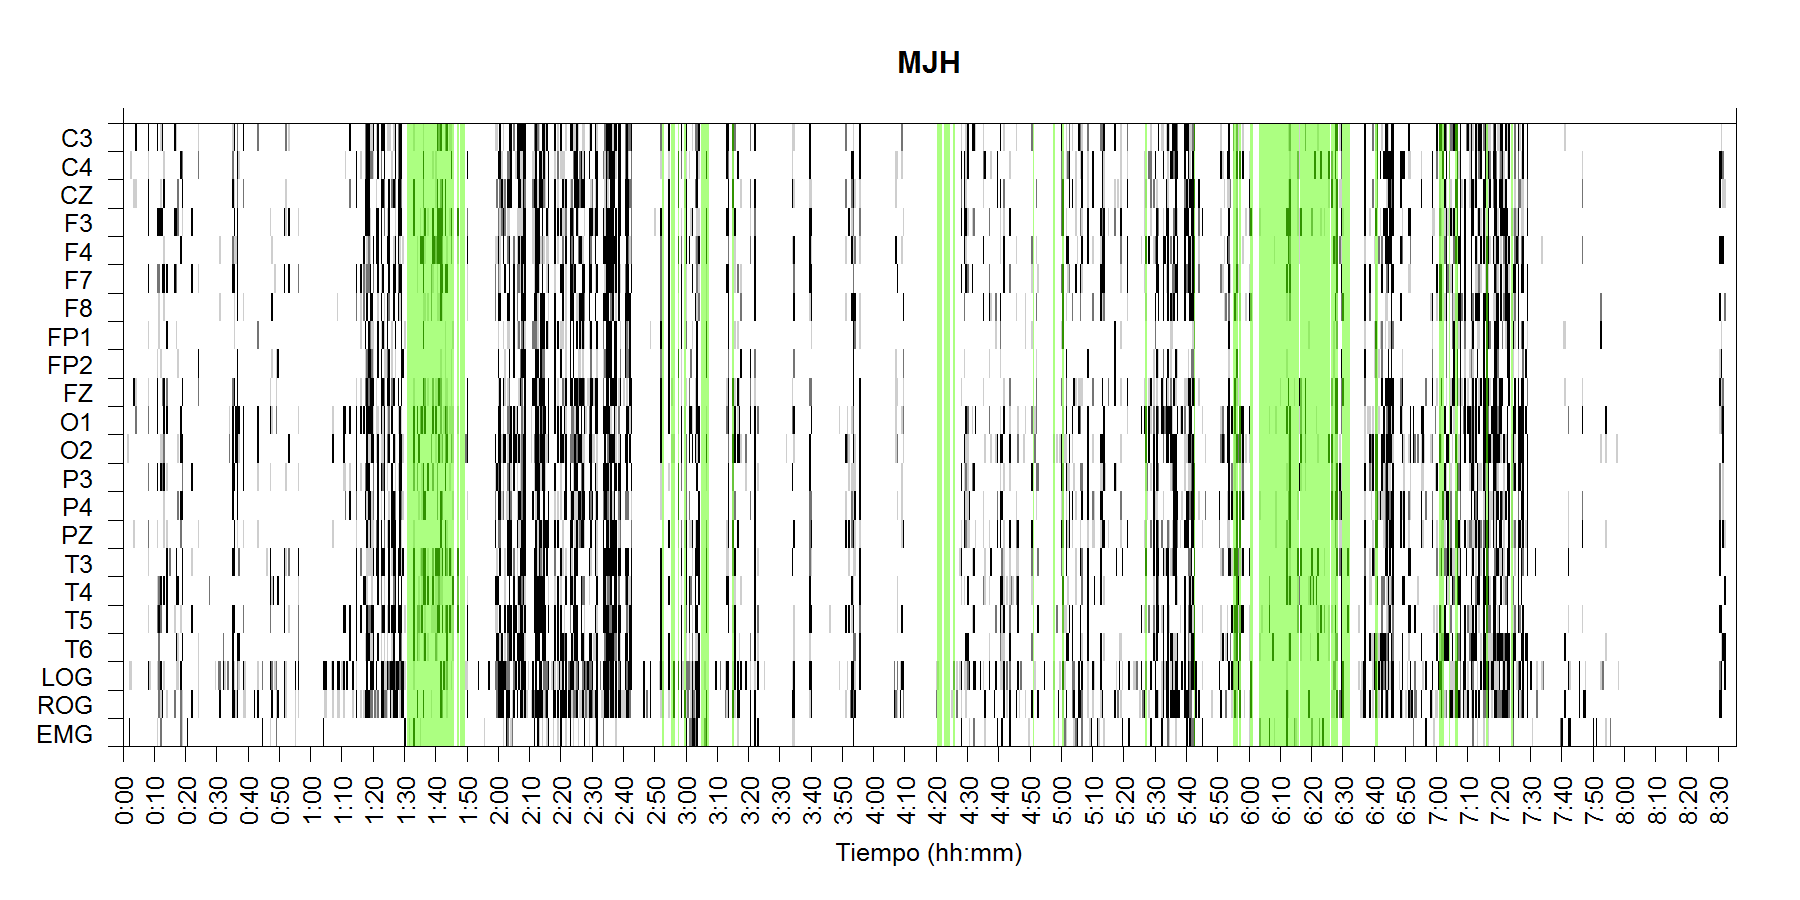
\includegraphics[width=\linewidth]
{./muypreeliminar170408/MJNNVIGILOS_est.png} 
\caption{Sujeto: MJH | Total \'epocas: 1032 | \'Epocas MOR: 127
%| Frecuencia de muestreo: 200 Hz
}
\label{grf:MJH}
\end{figure}

%%%%%%%%%%%%%%%%%%%%%%%%%%%%%%%%%%%%%%%%%%%%%%%%%

\begin{figure}
\centering
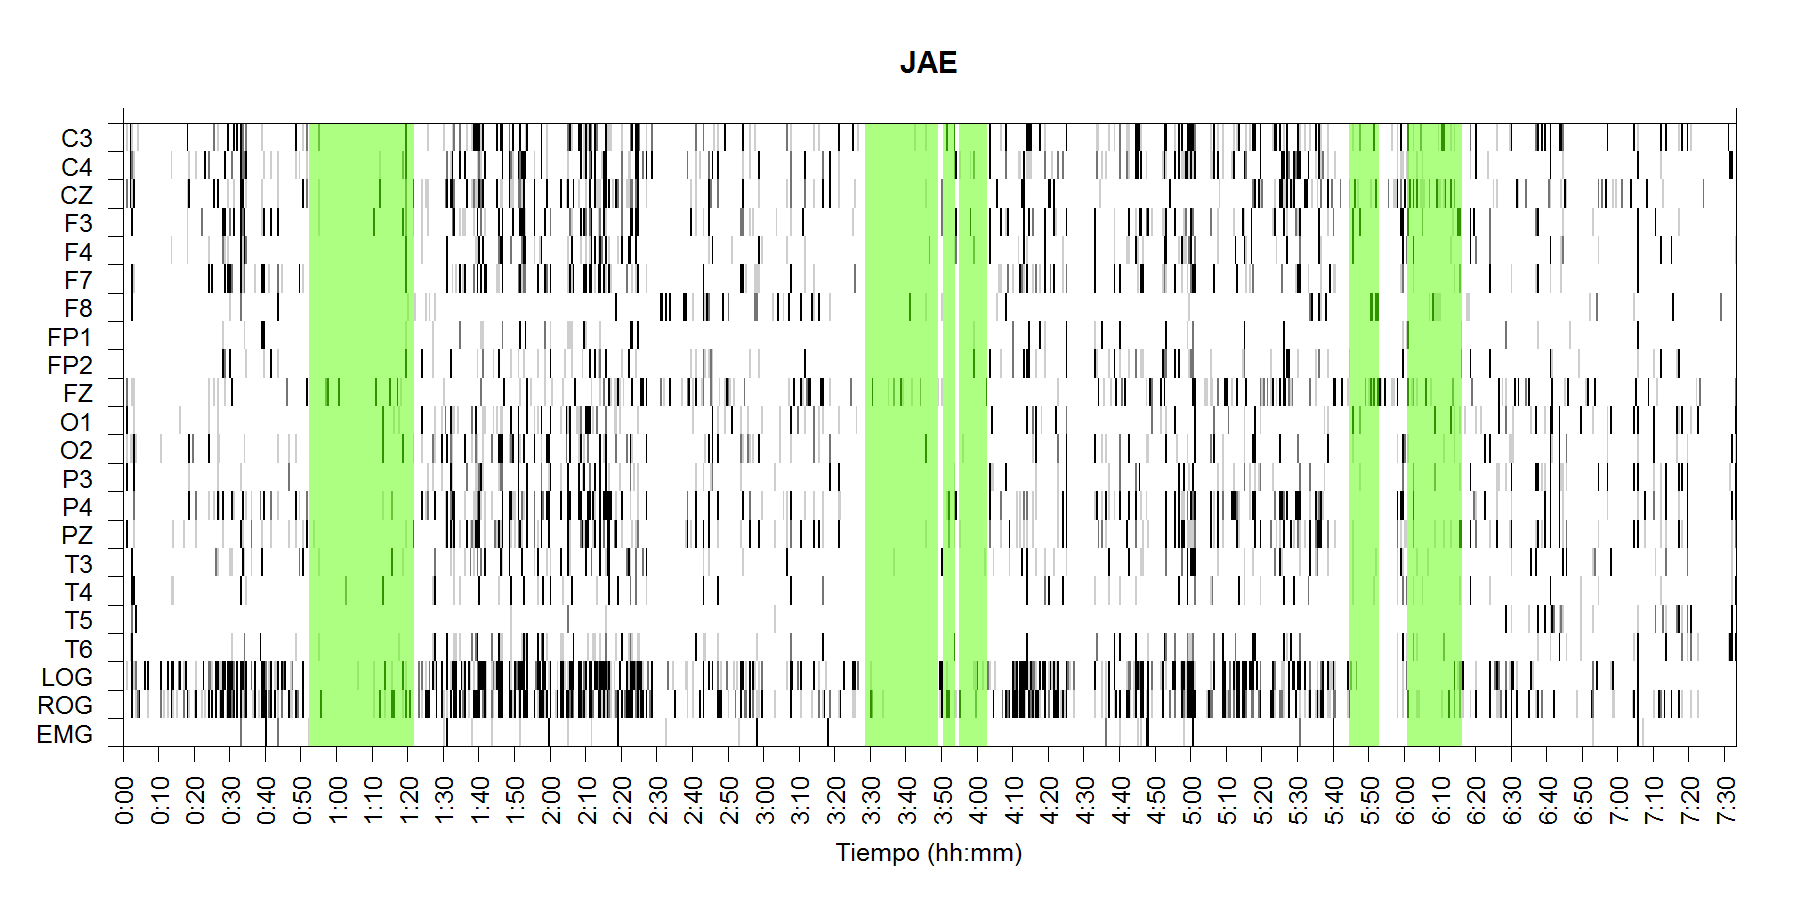
\includegraphics[width=\linewidth]
{./muypreeliminar170408/JANASUE_est.png} 
\caption{Sujeto: JAE | Total \'epocas: 907 | \'Epocas MOR: 171
%| Frecuencia de muestreo: 200 Hz
}
\label{grf:JAE}
\end{figure}

%%%%%%%%%%%%%%%%%%%%%%%%%%%%%%%%%%%%%%%%%%%%%%%%%

\begin{figure}
\centering
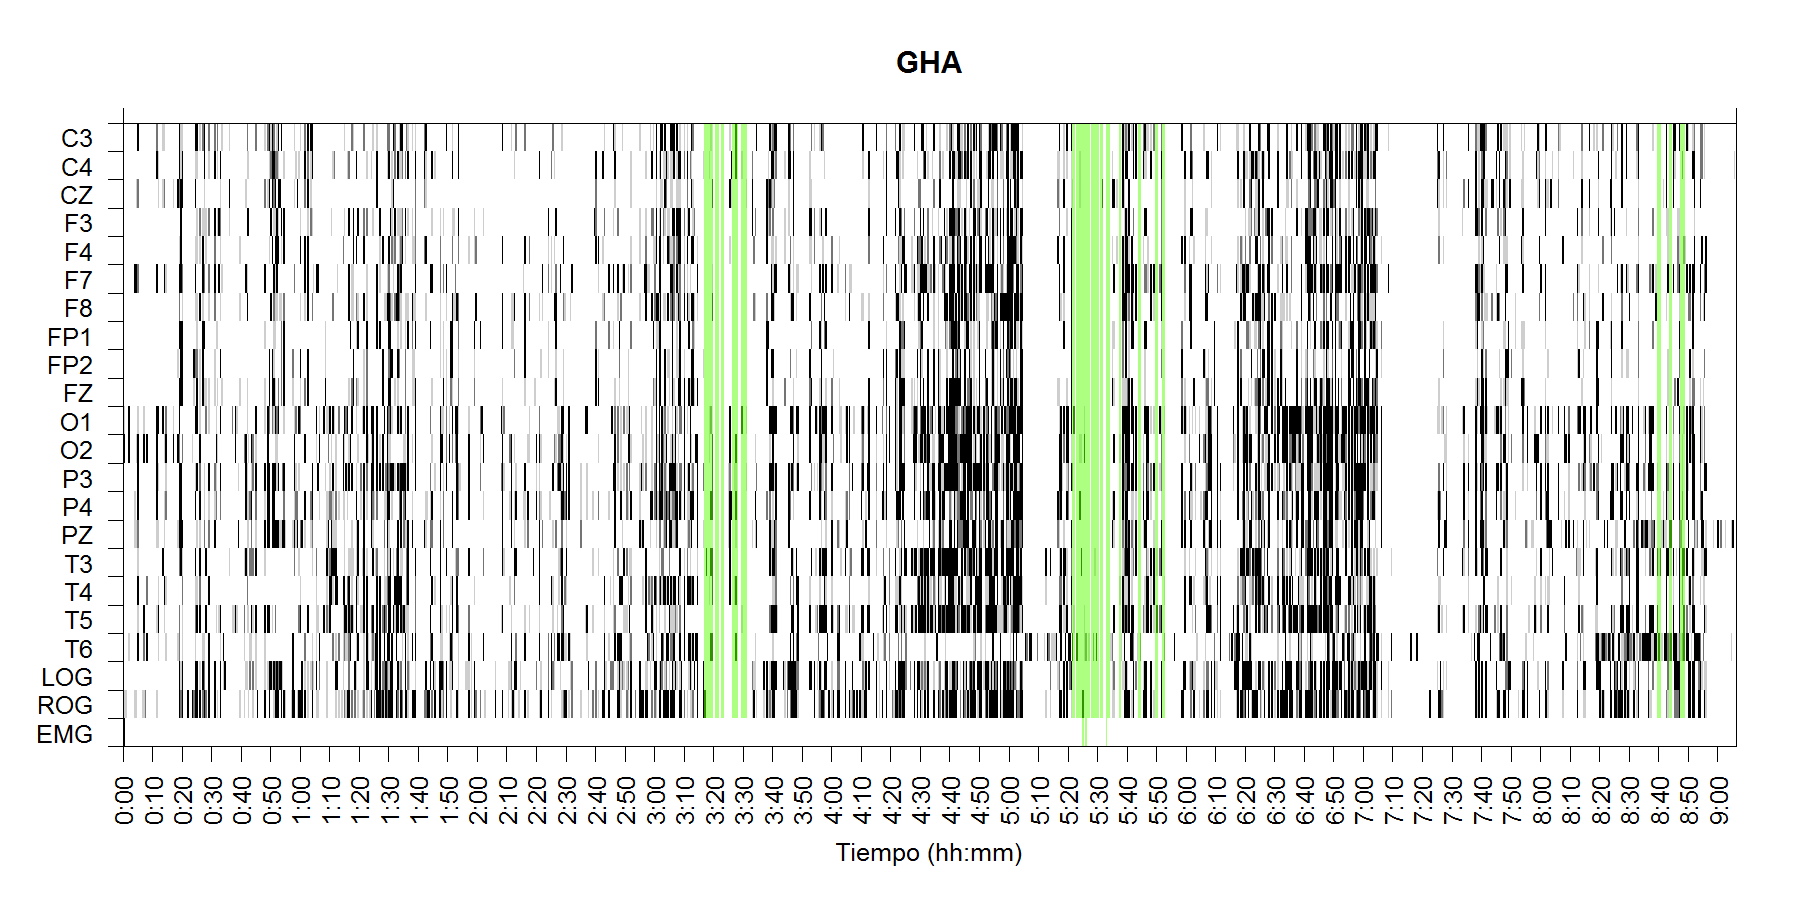
\includegraphics[width=\linewidth]
{./muypreeliminar170408/GH24031950SUENNO_est.png} 
\caption{Sujeto: GHA | Total \'epocas: 1093 | \'Epocas MOR: 55
%| Frecuencia de muestreo: 200 Hz
}
\label{grf:GHA}
\end{figure}

%%%%%%%%%%%%%%%%%%%%%%%%%%%%%%%%%%%%%%%%%%%%%%%%%

\begin{figure}
\centering
\includegraphics[width=\linewidth]
{./muypreeliminar170408/.png} 
\caption{Sujeto: MJH | Total \'epocas: 1032 | \'Epocas MOR: 127
%| Frecuencia de muestreo: 200 Hz
}
\label{grf:MFGR}
\end{figure}

%%%%%%%%%%%%%%%%%%%%%%%%%%%%%%%%%%%%%%%%%%%%%%%%%

\begin{figure}
\centering
{./muypreeliminar170408/.png} 
{./complementario170409/MJNNVIGILOS_est.png} 
\caption{Sujeto: MJH | Total \'epocas: 1032 | \'Epocas MOR: 127
%| Frecuencia de muestreo: 200 Hz
}
\label{grf:CLO}
\end{figure}

%%%%%%%%%%%%%%%%%%%%%%%%%%%%%%%%%%%%%%%%%%%%%%%%%

\begin{figure}
\centering
\includegraphics[width=\linewidth]
{./muypreeliminar170408/.png} 
\caption{Sujeto: MJH | Total \'epocas: 1032 | \'Epocas MOR: 127
%| Frecuencia de muestreo: 200 Hz
}
\label{grf:RLO}
\end{figure}

%%%%%%%%%%%%%%%%%%%%%%%%%%%%%%%%%%%%%%%%%%%%%%%%%

\begin{figure}
\centering
\includegraphics[width=\linewidth]
{./muypreeliminar170408/.png} 
\caption{Sujeto: MJH | Total \'epocas: 1032 | \'Epocas MOR: 127
%| Frecuencia de muestreo: 200 Hz
}
\label{grf:RRU}
\end{figure}

%%%%%%%%%%%%%%%%%%%%%%%%%%%%%%%%%%%%%%%%%%%%%%%%%

\begin{figure}
\centering
\includegraphics[width=\linewidth]
{./muypreeliminar170408/.png} 
\caption{Sujeto: MJH | Total \'epocas: 1032 | \'Epocas MOR: 127
%| Frecuencia de muestreo: 200 Hz
}
\label{grf:JGZ}
\end{figure}

%%%%%%%%%%%%%%%%%%%%%%%%%%%%%%%%%%%%%%%%%%%%%%%%%

\begin{figure}
\centering
\includegraphics[width=\linewidth]
{./muypreeliminar170408/.png} 
\caption{Sujeto: MJH | Total \'epocas: 1032 | \'Epocas MOR: 127
%| Frecuencia de muestreo: 200 Hz
}
\label{grf:FGH}
\end{figure}

%%%%%%%%%%%%%%%%%%%%%%%%%%%%%%%%%%%%%%%%%%%%%%%%%

\begin{figure}
\centering
\includegraphics[width=\linewidth]
{./muypreeliminar170408/.png} 
\caption{Sujeto: MJH | Total \'epocas: 1032 | \'Epocas MOR: 127
%| Frecuencia de muestreo: 200 Hz
}
\label{grf:MGG}
\end{figure}

%%%%%%%%%%%%%%%%%%%%%%%%%%%%%%%%%%%%%%%%%%%%%%%%%

\begin{figure}
\centering
\includegraphics[width=\linewidth]
{./muypreeliminar170408/.png} 
\caption{Sujeto: MJH | Total \'epocas: 1032 | \'Epocas MOR: 127
%| Frecuencia de muestreo: 200 Hz
}
\label{grf:EMT}
\end{figure}

%%%%%%%%%%%%%%%%%%%%%%%%%%%%%%%%%%%%%%%%%%%%%%%%%%%%%%%%%%%%%%%%%%%%%%%%%%%%%%%%%%%%%%%%%%%%%%%%%%%
%%%%%%%%%%%%%%%%%%%%%%%%%%%%%%%%%%%%%%%%%%%%%%%%%%%%%%%%%%%%%%%%%%%%%%%%%%%%%%%%%%%%%%%%%%%%%%%%%%%

%%\begin{SidewaysFigure}
%%\centering
%%\includegraphics[width=\linewidth]
%%{./grafiquitos170404/VCNNS1_est.png} 
%%\caption{Sujeto: VCR | Total \'epocas: 2584 | \'Epocas MOR: 200
%%%| Frecuencia de muestreo: 200 Hz
%%}
%%\label{VCR}
%%\end{SidewaysFigure}
%%
%%%%%%%%%%%%%%%%%%%%%%%%%%%%%%%%%%%%%
%%%%%%%%%%%%%%%%%%%%%%%%%%%%%%%%%%%%%
%%
%%\begin{SidewaysFigure}
%%\centering
%%\includegraphics[width=\linewidth]
%%{./grafiquitos170404/MJNNVIGILOS_est.png} 
%%\caption{Sujeto: MJH | Total \'epocas: 1032 | \'Epocas MOR: 127
%%%| Frecuencia de muestreo: 200 Hz
%%}
%%\label{MJH}
%%\end{SidewaysFigure}
%%
%%%%%%%%%%%%%%%%%%%%%%%%%%%%%%%%%%%%%
%%%%%%%%%%%%%%%%%%%%%%%%%%%%%%%%%%%%%
%%
%%\begin{SidewaysFigure}
%%\centering
%%\includegraphics[width=\linewidth]
%%{./grafiquitos170404/JANASUE_est.png} 
%%\caption{Sujeto: JAE | Total \'epocas: 907 | \'Epocas MOR: 171
%%%| Frecuencia de muestreo: 200 Hz
%%}
%%\label{JAE}
%%\end{SidewaysFigure}
%%
%%%%%%%%%%%%%%%%%%%%%%%%%%%%%%%%%%%%%
%%%%%%%%%%%%%%%%%%%%%%%%%%%%%%%%%%%%%
%%
%%\begin{SidewaysFigure}
%%\centering
%%\includegraphics[width=\linewidth]
%%{./grafiquitos170404/GH24031950SUENO_est.png} 
%%\caption{Sujeto: GHA | Total \'epocas: 3281 | \'Epocas MOR: 134
%%%| Frecuencia de muestreo: 200 Hz
%%}
%%\label{GHA}
%%\end{SidewaysFigure}
%%
%%%%%%%%%%%%%%%%%%%%%%%%%%%%%%%%%%%%%
%%%%%%%%%%%%%%%%%%%%%%%%%%%%%%%%%%%%%
%%
%%\begin{SidewaysFigure}
%%\centering
%%\includegraphics[width=\linewidth]
%%{./grafiquitos170404/GURM251148SUE_est.png} 
%%\caption{Sujeto: MFGR | Total \'epocas: 2466 | \'Epocas MOR: 267
%%%| Frecuencia de muestreo: 200 Hz
%%}
%%\label{MHGR}
%%\end{SidewaysFigure}
%%
%%%%%%%%%%%%%%%%%%%%%%%%%%%%%%%%%%%%%
%%%%%%%%%%%%%%%%%%%%%%%%%%%%%%%%%%%%%
%%
%%\begin{SidewaysFigure}
%%\centering
%%\includegraphics[width=\linewidth]
%%{./grafiquitos170404/CLMN10SUE_est.png} 
%%\caption{Sujeto: CLO | Total \'epocas: 944 | \'Epocas MOR: 132
%%%| Frecuencia de muestreo: 200 Hz
%%}
%%\label{CLO}
%%\end{SidewaysFigure}
%%
%%%%%%%%%%%%%%%%%%%%%%%%%%%%%%%%%%%%%
%%%%%%%%%%%%%%%%%%%%%%%%%%%%%%%%%%%%%
%%
%%\begin{SidewaysFigure}
%%\centering
%%\includegraphics[width=\linewidth]
%%{./grafiquitos170404/RLMN10SUE_est.png} 
%%\caption{Sujeto: RLO | Total \'epocas: 846 | \'Epocas MOR: 99
%%%| Frecuencia de muestreo: 200 Hz
%%}
%%\label{RLO}
%%\end{SidewaysFigure}
%%
%%%%%%%%%%%%%%%%%%%%%%%%%%%%%%%%%%%%%
%%%%%%%%%%%%%%%%%%%%%%%%%%%%%%%%%%%%%
%%
%%\begin{SidewaysFigure}
%%\centering
%%\includegraphics[width=\linewidth]
%%{./grafiquitos170404/RRMNS_est.png} 
%%\caption{Sujeto: RRU | Total \'epocas: 1244 | \'Epocas MOR: 114
%%%| Frecuencia de muestreo: 200 Hz
%%}
%%\label{RRU}
%%\end{SidewaysFigure}
%%
%%%%%%%%%%%%%%%%%%%%%%%%%%%%%%%%%%%%%
%%%%%%%%%%%%%%%%%%%%%%%%%%%%%%%%%%%%%
%%
%%\begin{SidewaysFigure}
%%\centering
%%\includegraphics[width=\linewidth]
%%{./grafiquitos170404/JGMN6SUE_est.png} 
%%\caption{Sujeto: JGZ | Total \'epocas: 1207 | \'Epocas MOR: 33
%%%| Frecuencia de muestreo: 200 Hz
%%}
%%\label{JGZ}
%%\end{SidewaysFigure}
%%
%%%%%%%%%%%%%%%%%%%%%%%%%%%%%%%%%%%%%
%%%%%%%%%%%%%%%%%%%%%%%%%%%%%%%%%%%%%
%%
%%\begin{SidewaysFigure}
%%\centering
%%\includegraphics[width=\linewidth]
%%{./grafiquitos170404/FGHSUE_est.png} 
%%\caption{Sujeto: FGH | Total \'epocas: 405 | \'Epocas MOR: 22
%%%| Frecuencia de muestreo: 200 Hz
%%}
%%\label{FGH}
%%\end{SidewaysFigure}
%%
%%%%%%%%%%%%%%%%%%%%%%%%%%%%%%%%%%%%%
%%%%%%%%%%%%%%%%%%%%%%%%%%%%%%%%%%%%%
%%
%%\begin{SidewaysFigure}
%%\centering
%%\includegraphics[width=\linewidth]
%%{./grafiquitos170404/MGNA5SUE_est.png} 
%%\caption{Sujeto: MGG | Total \'epocas: 1030 | \'Epocas MOR: 166
%%%| Frecuencia de muestreo: 200 Hz
%%}
%%\label{MGG}
%%\end{SidewaysFigure}
%%
%%%%%%%%%%%%%%%%%%%%%%%%%%%%%%%%%%%%%
%%%%%%%%%%%%%%%%%%%%%%%%%%%%%%%%%%%%%
%%
%%\begin{SidewaysFigure}
%%\centering
%%\includegraphics[width=\linewidth]
%%{./grafiquitos170404/EMNNS_est.png} 
%%\caption{Sujeto: EMT | Total \'epocas: 555 | \'Epocas MOR: 47
%%%| Frecuencia de muestreo: 200 Hz
%%}
%%\label{EMT}
%%\end{SidewaysFigure}

%%%%%%%%%%%%%%%%%%%%%%%%%%%%%%%%%%%%
%%%%%%%%%%%%%%%%%%%%%%%%%%%%%%%%%%%%
%
%\begin{SidewaysFigure}
%\centering
%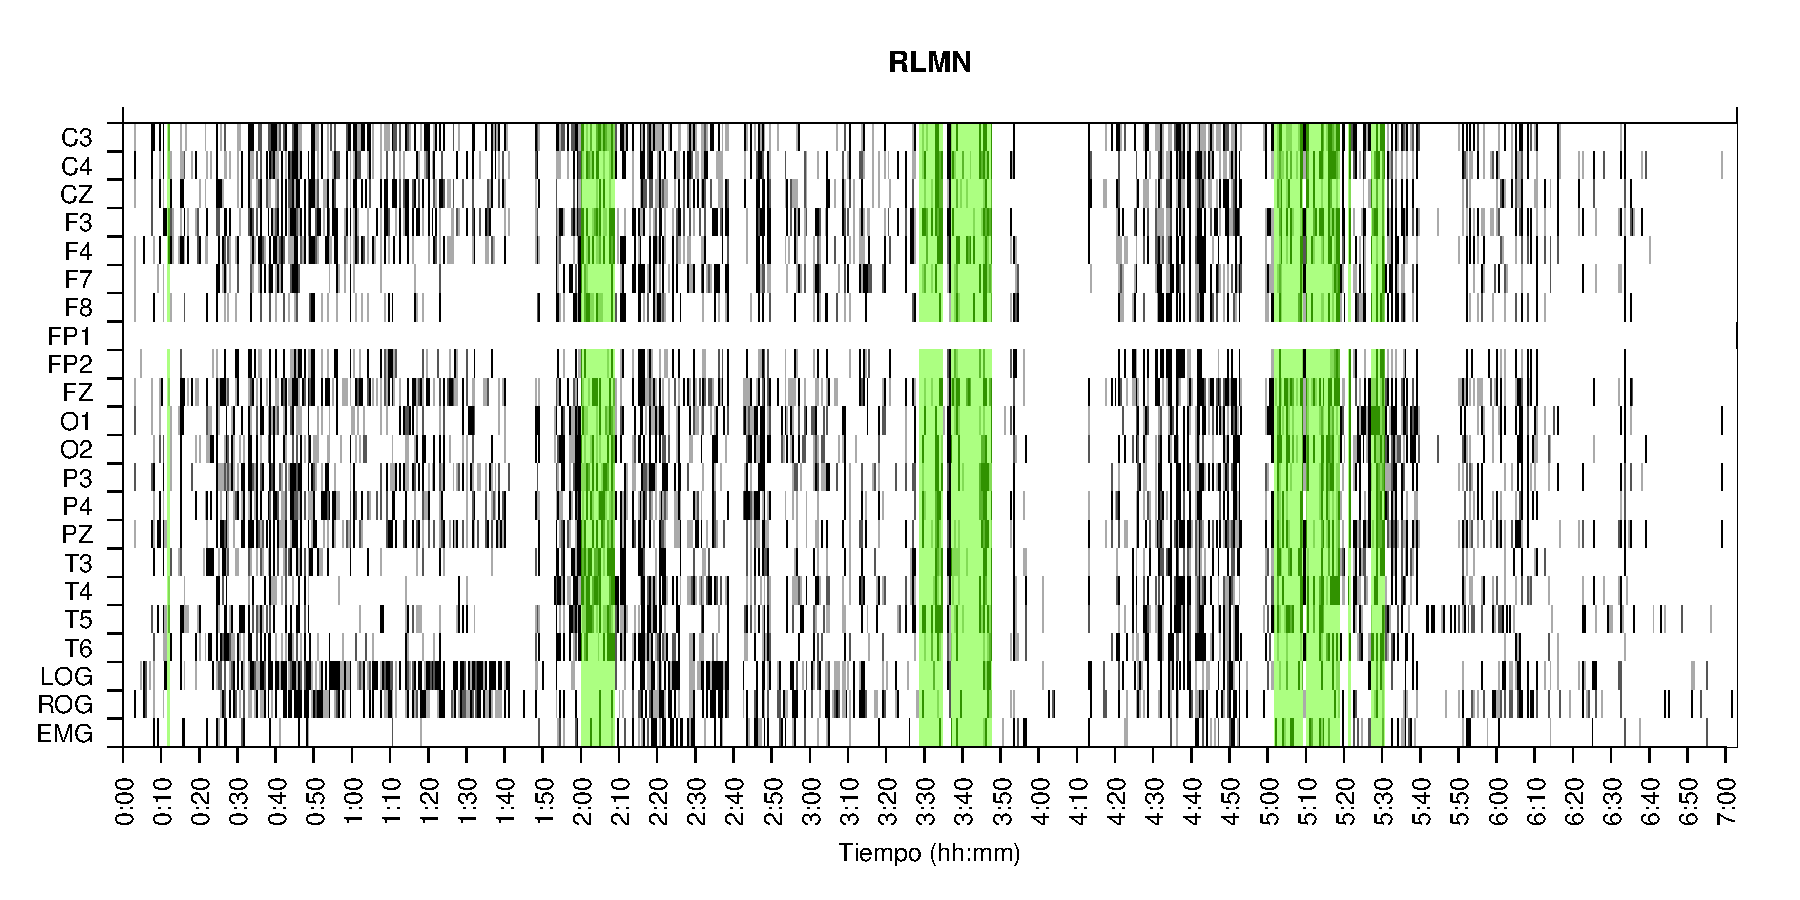
\includegraphics[width=\linewidth]{./material_bonito170220/RLMN10SUE_99_mor99_tot846_est_total.pdf} 
%\caption{Sujeto: RLMN | Total \'epocas: 846 | \'Epocas MOR: 99}
%%\label{primera}
%\end{SidewaysFigure}
%\begin{SidewaysFigure}
%\centering
%\includegraphics[width=\linewidth]
%{./material_bonito170220/RLMN10SUE_99_mor99_tot99_est_mor.pdf} 
%\caption{Sujeto: RLMN | \'Epocas MOR: 99 | (\'Unicamente \'epocas MOR)}
%%\label{primera}
%\end{SidewaysFigure}
%
%\begin{figure}
%\centering
%\includegraphics[width=\linewidth]
%{./material_bonito170220/porcentaje_bis/RLMN10SUE_99_846_1_bar_porcentaje.pdf} 
%\caption{Sujeto: RLMN | Porcentaje de \'epocas \textit{posiblemente estacionarias}}
%\end{figure}
%
%%%%%%%%%%%%%%%%%%%%%%%%%%%%%%%%%%%%
%%%%%%%%%%%%%%%%%%%%%%%%%%%%%%%%%%%%

%%%%%%%%%%%%%%%%%%%%%%%%%%%%%%%%%%%%%%%%%%%%%%%%%%%%%%%%%%%%%%%%%%%%%%%%%%%%%%%%%%%%%%%%%%%%%%%%%%%
%%%%%%%%%%%%%%%%%%%%%%%%%%%%%%%%%%%%%%%%%%%%%%%%%%%%%%%%%%%%%%%%%%%%%%%%%%%%%%%%%%%%%%%%%%%%%%%%%%%